\documentclass[11pt,a4paper]{article}

\usepackage[margin=1in, paperwidth=8.3in, paperheight=11.7in]{geometry}
\usepackage{amsmath,amsfonts,fancyhdr,bbm,graphicx,tikz}
\usepackage{float,hyperref}
\usetikzlibrary{automata,positioning}
\graphicspath{ {img/} }
\usepackage[section,nohyphen]{DomH}
\headertitle{Applied Data Science - Notes}

\begin{document}

\title{Applied Data Science - Notes}
\author{Dom Hutchinson}
\date{\today}
\maketitle

\tableofcontents\newpage

\section{Introduction}\label{sec_introduction}

  \begin{remark}{Types of Data}
    Data comes in many forms including, but not limited to, the following
    \begin{itemize}
      \item Dense \& Sparse data.
      \item Structured/Relational Data.
      \item Numerical; Categorical; Ordinal; or Boolean.
      \item Test (Emails, Tweets, Articles).
      \item Records (User-Level Data, Timestamped Event Data, Log Files).
      \item Geo-Based Location Data.
      \item Data-Time Data.
      \item Network Data.
      \item Sensor Data.
      \item Images and Video.
      \item Audio and Music.
    \end{itemize}
  \end{remark}

  \begin{remark}{Big \& Small Data}
    Whether a dataset is big or small depends on the computational-resources available, and thus will vary over time. Here are some ways to evaluate this
    \begin{center}
      \begin{tabular}{l|p{6cm}|p{6cm}}
        &\textbf{Big Data}&\textbf{Small Data}\\\hline
        \textit{Data Condition}&Always unstructured, not read for analysis, many relational database tables that need to be merged.&Ready for analysis, flat file, no need to merge tables.\\\hline
        \textit{Location}&Cloud, offshore, SQL server etc.&Database, local PC.\\\hline
        \textit{Data Size}&Over 50k variables, over 50k individuals, random samples, unstructured&File that is in a spreadsheet, that can be viewed on a few sheets of paper.\\\hline
        \textit{Data Purpose}&No intended purpose.&Intended purpose for data collection.
      \end{tabular}
    \end{center}
  \end{remark}

  \begin{remark}{What is Data Science?}
    Data-Driven Science. An interdisciplinary field about scientific processes and systems to extract knowledge or insights from data in various forms.
    \par Data science incorporates fields from: Mathematics, Computer Science; \&, Domain Expertise.
  \end{remark}

  \begin{remark}{Motivating Applications}
    Data science is motivated by its applications. Here are some examples of such applications
    \begin{itemize}
      \item \textit{Amazon} use recommender systems to suggest products to customers.
      \item \textit{Energy Companies} use data science to try and predict future usage of customers, so that resources can be applied efficiently.
      \item \textit{Agriculture} use sensors in fields to collect data in order to monitor crops and predict weather.
      \item \textit{Healthcare} use sensors in homes to monitor the health of people over long periods of time (especially when the person cannot go to the hospital).
    \end{itemize}
  \end{remark}

  \begin{figure}[H]
    \centering
    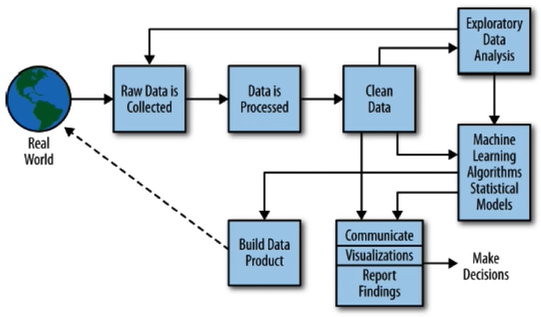
\includegraphics[width=.7\textwidth]{DataSciencePipeline.PNG}
    \caption{The pipeline for approaching problems in data science.}
    \label{fig_DataSciencePipeline}
  \end{figure}

  \begin{proposition}{Data Science Pipeline}
    See \texttt{Figure \ref{fig_DataSciencePipeline}} for a pipeline for approaching data science problems.
  \end{proposition}

\section{Data Ingress \& Pre-Processing}\label{sec_data_ingress}

\subsection{Data Structures}\label{sec_data_structures}

  \begin{proposition}{Native Python Data Structures}
    Here are some data structures which are native to python and are popular in data science
    \begin{itemize}
      \item \texttt{list} - List of elements of varying types.
      \item \texttt{set} - List of unique elements of varying types.
      \item \texttt{dict} - Key-Value pairings.
    \end{itemize}
  \end{proposition}

  \begin{proposition}{Non-Native Python Data Structures}
    Here are some data structures which are \underline{not} native to python but are popular in data science.
    \begin{itemize}
      \item \texttt{np.array}.
      \item \texttt{pandas.DataFrame}.
    \end{itemize}
  \end{proposition}

\subsection{Data Formats}\label{sec_data_formats}

  \begin{definition}{Object Persistence}
    \textit{Object Persistence} is the process of ensuring that the objects which are created are kept through multiple sessions. This comes in two stages
    \begin{enumerate}
      \item \textit{Serialisation} - Translating data structures or objects from memory into a format which can be stored.
      \item \textit{Deserialisation} - The inverse. Translating data structures which have been stored, into memory.
    \end{enumerate}
  \end{definition}

  \begin{remark}{Bespoke Serialisation \& Deserialisation}
    Bespoke serialisation and deserialisation methods can be crafted manually. (e.g. Instantiating an output file; Writing each element of a list to a different line in the file; Closing the file.)
    \par However, there are limitations to bespoke methods:
    \begin{itemize}
      \item Methods are specific to each use case (not standardised).
      \item Methods may not be robust.
      \item Methods require testing against many test cases.
      \item Object metadata is not encoded.
    \end{itemize}
    These limitations are rarely a problem in very controlled environments.
  \end{remark}

  \begin{definition}{Comma-Separated Values (CSV)}
    \textit{Comma-Separated Values} (CSV) files are well suited to tabular data (inc. matrices). Each line of a \textit{CSV File} stores one row of the table, and each element in a row is separated by a comma.
    \par \textit{CSV Files} are generally very readable, as well as time- and space-efficient for tabular data.
  \end{definition}

  \begin{remark}{Using CSV Files}
    As \textit{CSV Files} are very popular, there are many library methods which can interact with them. Including reading \& writing to and from memory (e.g. \texttt{pandas.read\_csv}).
  \end{remark}

  \begin{definition}{JavaScript Object Notation (JSON)}
    \textit{JavaScript Object Notation}\footnote{JSON is not just compatible with JavaScript and is common for many languages \& APIs} (JSON) is a standardised syntax for storing \& exchanging data, used for serialisation. JSON uses text files which are human-readable and \texttt{dict}-like (i.e. have value-key pairs). JSON is designed to be simple so is a very robust language \& suits many purposes.\footnote{\url{https://jsonlint.com/} is a useful site for JSON validation.}
    \par Limitations of JSON are that a specific conversion process may be required to convert a JSON file into objects in memory, and JSON files can become large due to key repetition.
  \end{definition}

  \begin{definition}{Hierarchical Data Format (HDF5)}
    \textit{Hierarchical Data Format} (HDF5) is a standardised format for serialisation. HDF5 is a binary format and tries to mimic  file system-like access. HDF5 files have the following three components
    \begin{enumerate}
      \item \textit{Datasets} - Array-like collections of data. Thousands of datasets can be stored in a single file, and can be categorised and tagged however you want.
      \item \textit{Groups} - Folder-like structures which groups datasets \& other groups.
      \item \textit{Metadata} - Information which pertains to all the datasets. (e.g. author, edit data \& version).
    \end{enumerate}
    \par HDF5 files are ideal for large numerical data sets, and can easily be manipulated by \texttt{numpy}. HDF5 files support a variety of transparent storage features (inc. compression, error-detection and chunked I/O), which \texttt{numpy.array} do not.\footnote{\url{http://docs.h5py.org/en/latest/quick.html} provides a quick-start guide to using HDF5 files in python.}
  \end{definition}

  \begin{proposition}{HDF5 files vs Traditional File Systems}
    There are a few key differences between \textit{HDF5 Files} and \textit{Traditional File Systems}.
    \begin{enumerate}
      \item \textit{HDF5 Files} are portable, as the entire structure is contained in the file independent of the underlying file system.\footnote{However, it does depend on the HDF5 library.}
      \item Datasets in \textit{HDF5 Files} are all homogeneous hyper-rectangular numerical arrays, whereas files in traditional file system can be anything.
      \item Metadata can be added to groups in \textit{HDF5 Files}. This is not possible in traditional file systems.
    \end{enumerate}
  \end{proposition}

  \begin{remark}{Other Standardised Serialisation Method}
    XML, \textit{Protocol Buffers} \& YAML are other popular standardised serialisation methods.
  \end{remark}

\subsection{Web-Scraping \& APIs}\label{sec_web_scraping_and_apis}

  \begin{remark}{Terms of Use}
    \textit{Web Scraping} should be done within the website's terms of use.
  \end{remark}

  \begin{definition}{Web Scraping}
    \textit{Web Scraping} is the practice of collecting data from websites. This can take many forms, but typically involves taking a raw webpage and parsing the desired data.
  \end{definition}

  \begin{proposition}{Approaching Web Scraping}
    To perform \textit{Web Scraping} successfully, you need a good idea of how a webpage is structure. Typically webpages are based around a \texttt{html} file, which are well structured\footnote{Webpages are often interpreted to have a tree structure, with each tag being a node}. Identifying combinations of tags, classes \& ids in the \texttt{html}  file can help locate the desired data.
    \par It is harder, sometimes impossible, to navigate poorly designed websites as they are less structured and inconsistent.
  \end{proposition}

  \begin{remark}{Tools for Web Scraping}
    \textit{Web Scraping} technologies need to be tolerant to several artefacts of real-world data (known as \textit{"wrangling"}) as-well-as errors in the website.
    \par Some popular tools for \textit{Web Scraping} are
    \begin{itemize}
      \item \texttt{BeautifulSoup} - A python library for parsing \texttt{XML} \& \texttt{HTML}.
      \item \texttt{scrapy} - A python library. Generally faster than \texttt{BeautifulSoup}.
      \item \texttt{Selenium} - A web-browser plugin, generally used to test web services.
    \end{itemize}
  \end{remark}

  \begin{definition}{Web APIs}
    \textit{Web APIs} greatly simplify \textit{Web Scraping} by provide a portal for explicit data acquisition, and are generally less prone to the issues which arise when \textit{Web Scraping}.\footnote{See \url{https://github.com/public-apis/public-apis} for a categorised list of public APIs.}
    \begin{itemize}
      \item The code running \textit{Web APIs} is optimised for data requesting \& retrieval. It does not waste time on visualisation or aesthetics. This means the bandwidth required for an \textit{API} request is much lower than for a similiar \textit{Web Scraping} process (As images etc. do not need to be loaded).
      \item \textit{Web API} querying is robust, reliable, well maintained and documented with a static schema (\texttt{HTML}-based \textit{Web Scraping} is not).
      \item \textit{Web APIs} use standardised \textit{Serialisation Tools} (e.g. JSON).
      \item \textit{Web APIs} have already extracted and organised the desired data, however this does mean the user can only access what the operator will allow. This is much better than \texttt{HTML}-based \textit{Web Scraping} where you rely upon fickle naming conventions of tags.
    \end{itemize}
  \end{definition}

  \begin{definition}{RESTful APIs}
    \textit{Representational State Transfer APIs} (REST/RESTful) are a popular form of \textit{Web API} and generally require an \textit{API Key} to access data.
    \par Request to \textit{RESTful APIs} generally involves constructing a URL which contains your keys and the parameters of your query.
  \end{definition}

  \begin{remark}{Regular Expression (RegEx)}
    \textit{Regular Expression} (ReGex) queries are useful for extracting data, either while web scraping or from API requests.\footnote{\url{http://pythex.org/} is a website which can perform \textit{RegEx}.} Python has the \texttt{re} library for \textit{RegEx} queries, two popular methods from this library are
    \begin{enumerate}
      \item \texttt{re.match} - Attempts to match a \textit{RegEx} pattern to the whole string.
      \item \texttt{re.search} - Searches for the \underline{first} occurrence of a \textit{RegEx} pattern in a string.
    \end{enumerate}
  \end{remark}

\section{Privacy}\label{sec_privacy}

\subsection{IRL Examples}\label{sec_privacy_examples}

  \begin{remark}{AOL Data Incident, 2006}
    In 2006, \textit{AOL Research} released to the public, for the purpose of research, a text file containing 20mn search terms from over 650k users, over a 3-month period.
    \par The users were anonymised in the in the data, but personally identifiable information was present in many of the search terms.
    \par \textit{AOL Research} retracted the document shortly after publishing.
  \end{remark}

  \begin{remark}{Netflix Prize, 2007}
    In 2007, \textit{Netflix} ran a competition where \$1mn was offered to anyone who was able to produce a system which outperformed their existing recommender system by at least 10\%.
    \par The training data offered by \textit{Netflix} contained <user,movie,date,grade> and customer ids were anonymised.
    \par It was later found that some users had their \textit{Netflix} and \textit{IMDb} accounts linked (so reviews were posted on both). This meant the training data could be partially de-anonymised. This led to lawsuits and \textit{Netflix} cancelling future competitions.
  \end{remark}

  \begin{remark}{Pay Attention}
    The moral of these examples is that you have to be really careful and diligent when anonymising data as there may be non-obvious ways for people to de-anonymise it. (Often through little fault of your own).
  \end{remark}

\subsection{Security \& Statistical Database}\label{sec_security_and_statistical_database}

  \begin{definition}{Statistical Database}
    A \textit{Statistical Database} is a database for statistics. They can come in several forms
    \begin{itemize}
      \item \textit{Tabular Data} - Tables with counts or magnitudes.
      \item \textit{Queryable Databases} - On-line databases which accept statistical queries (e.g. min, max, sum etc.)
      \item \textit{Microdata} - Files where each record contains information about an individual.
    \end{itemize}
  \end{definition}

  \begin{remark}{Privacy Trade-Off}
    \textit{Statistical Databases} have to trade-off privacy and functionality. Generally, more privacy means less functionality.
  \end{remark}

  \begin{definition}{Identifiers}
    \textit{Identifiers} are attributes that unambiguously identify someone (e.g. passport number, NI number, name etc.)
  \end{definition}

  \begin{definition}{Quasi-Identifiers}
    \textit{Quasi-Identifiers} are attributes which identify someone, but there is some ambiguity. Often, having multiple \textit{Quasi-Identifiers} are enough to confidently identify someone. (e.g. address, age, gender).
  \end{definition}

  \begin{definition}{Confidential Attributes}
    \textit{Confidential Attributes} are attributes which contain sensitive information about an individual (e.g. salary, religion, medical conditions etc.)
  \end{definition}

  \begin{definition}{Non-Confidential Attributes}
    \textit{Non-Confidential Attributes} are attributes which do \underline{not} contain sensitive information about an individual.
  \end{definition}

  \begin{remark}{Anonymisation, Identifiers \& Quasi-Identifiers}
    When anonymising a data set:
    \begin{itemize}
      \item \textit{Identifiers} need to be suppressed from the data sets (i.e. removed).
      \item \textit{Quasi-Identifiers} hold disclosure risk as they can often not be suppress due their high analytical value, but can often be linked with other non-anonymised datasets to de-anonymise your dataset.
    \end{itemize}
  \end{remark}

  \begin{definition}{Attribute Disclosure}
    \textit{Attribute Disclousure} is when the value of a confidential attribute is made available, and in doing so the individual is easier to identifier (compared to the value not being disclosed).
  \end{definition}

  \begin{definition}{Identity Disclosure}
    \textit{Identity Disclosure} is when an entire record in an anonymised data set can be linked with that individual's identity.
  \end{definition}

  \begin{definition}{Membership Disclosure}
    \textit{Membership Disclosure} is whether or not data about an individual is contained in a dataset.
  \end{definition}

  \begin{definition}{External Attack on a Table}
    An \textit{External Attack} on a table occurs when another dataset is released which contains data which comprises more table, or can be combined with your table to comprise others.
  \end{definition}

  \begin{definition}{Internal Attack on a Table}
    An \textit{Internal Attack} on a table occurs when those within the table (i.e. with access to it and know which data represents them) are able to deduce which data belongs to other people by a process of elimination.
    \par Only really possible when the table has few respondents.
  \end{definition}

  \begin{definition}{Dominance Attack on a Table}
    An \textit{Internal Attack} on a table occurs a (or a few) respondents dominate the contribution in a particular cell of a magnitude table, these \textit{Dominant Respondents} are then able to upper-bound the contributions from the rest due it being easier to differentiate other users from them.
  \end{definition}

  \begin{proposition}{Combatting Table Attacks}
    There are two main approaches to combatting \textit{Table Attacks}
    \begin{enumerate}
      \item \textit{Non-Perturbative} techniques which do \underline{not} modify the values in the cells, but they may suppress or recode them (e.g. cell suppression, recoding of categorical attributes).
      \item \textit{Perturbative} techniques do modify the values in the cells (e.g. controlled rounding).
    \end{enumerate}
  \end{proposition}

  \begin{proposition}{Combatting Database Attacks}
    There are three main approaches to combatting attacks on databases, all focused around adjusting/controlling queries
    \begin{enumerate}
      \item \textit{Query Input Perturbation} - Perturbation is applied to records on which queries are computed.
      \item \textit{Query Output Perturbation} - Perturbation is applied to the results of a query.
      \item \textit{Query Restriction} - The database refuses certain queries.
      \item \textit{Camoflage} - Returns answers which have been made non-exact in some deterministic fashion.
    \end{enumerate}
  \end{proposition}

  \begin{remark}{Differential Attack\footnote{Not proper name.}}
    Suppose you know that someone is going to be changing doctors soon (and thus will be removed from the doctors database), if you copied the database before and after this person moves you could likely deduce details about the individual by comparing the two versions.
    \par How do we prevent this?
  \end{remark}

  \begin{definition}{Differential Privacy}
    Consider a learner implements a summary statistic $A$ (e.g. sum of all elements); an adversary proposes two datasets $S$ and $S'$ which differ by only one row; and a test set $Q$. The learner wants the summary statistic to have the same value if only one row has changed.
    \par Summary statistic $A$ is \textit{$\varepsilon$-Differentially Private} iff
    \[ \left|\ln\left(\frac{\prob(A(S)\in Q)}{\prob(A(S')\in Q)}\right)\right|\leq\varepsilon \]
    Note that \textit{Differential Privacy} is a condition on the release mechanism of the data $A$, not on the data $S,S'$ itself.
  \end{definition}

  \begin{remark}{Differential Privacy in Practice}
    In practice we avoid differential privacy issues by adding noise to our responses (either to all responses, or incorrectly responding to some queries).
  \end{remark}

\subsection{$k$-Anonymity}\label{sec_k_anonymity}

  \begin{definition}{$k$-Anonymity}
    A dataset satisfies \textit{$k$-Anonymity} if each combination of values of \textit{Quasi-Identifier Attributes} in the table are shared by at least $k$ records.
    \par Measuring \textit{$k$-Anonymity} requires a brute force approach which compares every pair of records in the table.
  \end{definition}

  \begin{proposition}{Achieving $k$-Anonymity}
    There are two main approaches to achieving \textit{$k$-Anonymity}:
    \begin{itemize}
      \item \textit{Suppression} - Replace the values of attributes with an asterisk.
      \item \textit{Generalisation} - Values of attributes are replaced with a broader category. (e.g. age-ranges rather than exact age)
    \end{itemize}
  \end{proposition}

  \begin{proposition}{$k$-Anonymity Attacks}
    \textit{$k$-Anonymity} does not protect against attribute disclosure attacks in general if the values of \textit{Confidential Attributes} are very similar in the group of $k$ records who share \textit{Quasi-Identifier} values.
    \par Here are two specific attacks that can happen
    \begin{itemize}
      \item \textit{Homogeneity Attack} - If all records in the set of $k$ identical records have the same \textit{Sensitive Value}, then the value can likely be predicted (and would comprise all $k$).
      \item \textit{Background Knowledge Attack} - If associations exist between one or more \textit{Quasi-Identifier Attributes} and a \textit{Sensitive Attribute} then the set of possible values of the \textit{Sensitive Attribute} is reduced.
    \end{itemize}
  \end{proposition}

  \begin{definition}{$l$-Diversity}
    \textit{$l$-Diversity} is an extension of \textit{$k$-Anonymity}.
    \par \textit{$l$-Diversity} requires that the values of all \textit{Confidential Attributes} within any group of $k$-anonymous records contain at least $l$ clearly distinct values.
  \end{definition}

  \begin{proposition}{Limitations of $l$-Diversity}
    Here are two limitations of \textit{$l$-Diversity}
    \begin{itemize}
      \item Not every value shows equal sensitivity. (A rare positive indicator for a disease may provide more information than a common negative indicator).
      \item It ensures diversity of sensitive values in each group, but it does not recognise that values may be semantically similar.
    \end{itemize}
  \end{proposition}

  \begin{definition}{$t$-Closeness}
    \textit{$t$-Closeness} requires that the distribution of the confidential attribute within a group of $k$ records is similar to the distribution of the confidential attribute in the entire data set (at most distance $t$ between the two distributions).
  \end{definition}

  \begin{remark}{Tools for Anonymisation}
    Here are three popular tools for anonymisation
    \begin{enumerate}
      \item \textit{ARX} - Applies $k$-anonymity, $l$-diversity and $t$-clossness in Java.
      \item \textit{Argus} - Creates safe microdata files.
      \item \textit{SdcMicro} - Provides disclosure control methods for anonymisation and risk-estimation.
    \end{enumerate}
  \end{remark}

\subsection{Other Approaches}\label{sec_other_approaches}

  \begin{definition}{Privacy-Preserving Data Mining, PPDM}
    \textit{Privacy-Preserving Data Mining} (PPDM) seeks privacy for the data's owner when several owners wish to co-operate without giving away their data to each other
  \end{definition}

  \begin{definition}{Private Information Retrieval}
    \textit{Private Information Retrieval} (PIR) seeks user privacy to allow the user of a database to retrieve information without the database knowing which item was retrieved.
  \end{definition}

\section{Storage \& Management}\label{sec_storage_and_management}

\section{Transformation \& Integration}\label{sec_transformation_and_integration}

\section{Exploration \& Visualisation}\label{sec_exploration_and_visualisation}

\section{Deployment}\label{sec_deployment}

\section{Sharing \& Privacy}\label{sec_sharing_and_privacy}

\end{document}
